\subsection{Scenario Anagrafiche}
\begin{figure}[H] 
    \centering 
    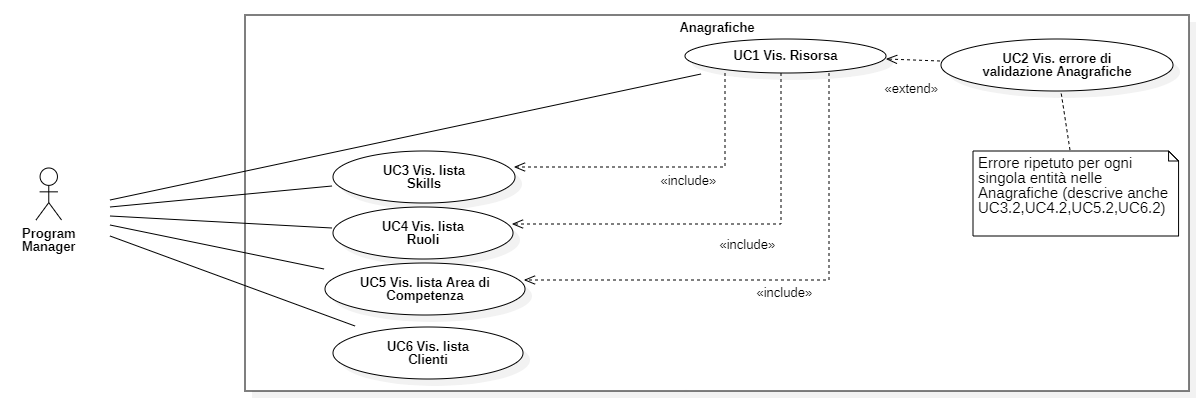
\includegraphics[width=1.1\columnwidth]{usecase/anagrafiche-general} 
    \caption{Casi d'Uso del scenario Anagrafiche}
\end{figure}

\subsubsection*{UC1 - Vis. Risorsa}

\begin{figure}[H] 
    \centering 
    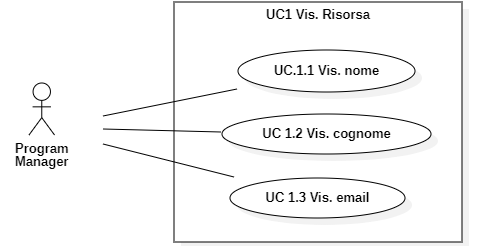
\includegraphics[width=0.6\columnwidth]{usecase/UC1} 
    \caption{Caso d'Uso 1 espanso}
\end{figure}

\begin{itemize}[label=$\circ$]
\item \textbf{Attore:} Program Manager;
\item \textbf{Descrizione:} il Program Manager può visualizzare una Risorsa;
\item \textbf{Precondizioni:} il richiedente è un Program Manager;
\item \textbf{Postcondizioni:} la Risorsa selezionata è visualizzabile dal Program Manager;
\item \textbf{Estensioni:} UC2;
\item \textbf{Inclusioni:} UC3, UC4, UC5.
\end{itemize}

\subsubsection*{UC1.1 - Vis. nome}
\begin{itemize}[label=$\circ$]
\item \textbf{Attore:} Program Manager;
\item \textbf{Descrizione:} il Program Manager può visualizzare il nome di una Risorsa;
\item \textbf{Precondizioni:} la Risorsa è visualizzabile dal Program Manager;
\item \textbf{Postcondizioni:} il Program Manager può visualizzare il nome della Risorsa selezionata;
\item \textbf{Estensioni:} il caso d'uso non ha estensioni;
\item \textbf{Inclusioni:} il caso d'uso non ha inclusioni.
\end{itemize}

\subsubsection*{UC1.2 - Vis. cognome}
\begin{itemize}[label=$\circ$]
\item \textbf{Attore:} Program Manager;
\item \textbf{Descrizione:} il Program Manager può visualizzare il cognome di una Risorsa;
\item \textbf{Precondizioni:}  la Risorsa è visualizzabile dal Program Manager;
\item \textbf{Postcondizioni:} il Program Manager può visualizzare il cognome della Risorsa selezionata;
\item \textbf{Estensioni:} il caso d'uso non ha estensioni;
\item \textbf{Inclusioni:} il caso d'uso non ha inclusioni.
\end{itemize}

\subsubsection*{UC1.3 - Vis. email}
\begin{itemize}[label=$\circ$]
\item \textbf{Attore:} Program Manager;
\item \textbf{Descrizione:} il Program Manager può visualizzare l'email di una Risorsa;
\item \textbf{Precondizioni:}  la Risorsa è visualizzabile dal Program Manager;
\item \textbf{Postcondizioni:} il Program Manager può visualizzare l'email della Risorsa selezionata;
\item \textbf{Estensioni:} il caso d'uso non ha estensioni;
\item \textbf{Inclusioni:} il caso d'uso non ha inclusioni.
\end{itemize}

\subsubsection*{UC2 - Vis. errore di validazione Anagrafiche}
\begin{itemize}[label=$\circ$]
\item \textbf{Attore:} Program Manager;
\item \textbf{Descrizione:} questo caso d'uso descrive anche UC3.2,UC4.2,UC5.2,UC6.2. Viene visualizzato un messaggio di errore in caso vengano eseguite funzionalità con dati non validi. Esso rappresenta errori di validazione nella richiesta fornita dall'utilizzatore;
\item \textbf{Precondizioni:} il Program Manager sta effettuando operazioni con dati non validi;
\item \textbf{Postcondizioni:} l'esecuzione della funzionalità è interrotta e viene visualizzato il messaggio di errore;
\item \textbf{Estensioni:} il caso d'uso non ha estensioni;
\item \textbf{Inclusioni:} il caso d'uso non ha inclusioni.
\end{itemize}

\subsubsection*{UC3 - Vis. lista Skill}
\begin{figure}[H] 
    \centering 
    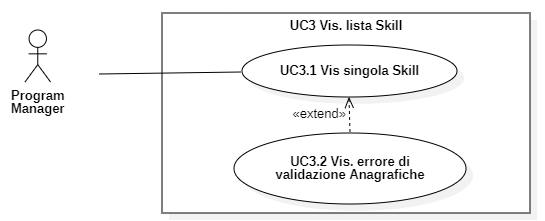
\includegraphics[width=0.6\columnwidth]{usecase/UC3} 
    \caption{Caso d'Uso 3 espanso}
\end{figure}
\begin{itemize}[label=$\circ$]
\item \textbf{Attore:} Program Manager;
\item \textbf{Descrizione:} il Program Manager può visualizzare la lista delle Skill;
\item \textbf{Precondizioni:} il richiedente è un Program Manager;
\item \textbf{Postcondizioni:} la lista delle Skill è visualizzabile dal Program Manager;
\item \textbf{Estensioni:} il caso d'uso non ha estensioni;
\item \textbf{Inclusioni:} il caso d'uso non ha inclusioni.
\end{itemize}

\subsubsection*{UC3.1 - Vis. singola Skill}
\begin{figure}[H] 
    \centering 
    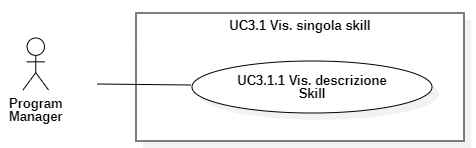
\includegraphics[width=0.6\columnwidth]{usecase/UC3.1} 
    \caption{Caso d'Uso 3.1 espanso}
\end{figure}
\begin{itemize}[label=$\circ$]
\item \textbf{Attore:} Program Manager;
\item \textbf{Descrizione:} il Program Manager può visualizzare una Skill;
\item \textbf{Precondizioni:} il richiedente è un Program Manager;
\item \textbf{Postcondizioni:} la Skill selezionata è visualizzabile dal Program Manager;
\item \textbf{Estensioni:} UC3.2;
\item \textbf{Inclusioni:} il caso d'uso non ha inclusioni.
\end{itemize}

\subsubsection*{UC3.1.1 - Vis. descrizione Skill}
\begin{itemize}[label=$\circ$]
\item \textbf{Attore:} Program Manager;
\item \textbf{Descrizione:} il Program Manager può visualizzare la descrizione di una Skill;
\item \textbf{Precondizioni:} la Skill è visualizzabile dal Program Manager;
\item \textbf{Postcondizioni:} il Program Manager può visualizzare la descrizione della Skill selezionata;
\item \textbf{Estensioni:} il caso d'uso non ha estensioni;
\item \textbf{Inclusioni:} il caso d'uso non ha inclusioni.
\end{itemize}

\subsubsection*{UC4 - Vis. lista Ruoli}
\begin{figure}[H] 
    \centering 
    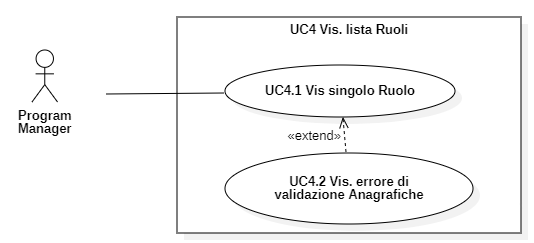
\includegraphics[width=0.6\columnwidth]{usecase/UC4} 
    \caption{Caso d'Uso 4 espanso}
\end{figure}
\begin{itemize}[label=$\circ$]
\item \textbf{Attore:} Program Manager;
\item \textbf{Descrizione:} il Program Manager può visualizzare la lista dei Ruoli;
\item \textbf{Precondizioni:} il richiedente è un Program Manager;
\item \textbf{Postcondizioni:} la lista dei Ruoli è visualizzabile dal Program Manager;
\item \textbf{Estensioni:} il caso d'uso non ha estensioni;
\item \textbf{Inclusioni:} il caso d'uso non ha inclusioni.
\end{itemize}

\subsubsection*{UC4.1 - Vis. singolo Ruolo}
\begin{figure}[H] 
    \centering 
    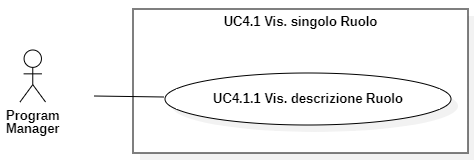
\includegraphics[width=0.6\columnwidth]{usecase/UC4.1} 
    \caption{Caso d'Uso 4.1 espanso}
\end{figure}
\begin{itemize}[label=$\circ$]
\item \textbf{Attore:} Program Manager;
\item \textbf{Descrizione:} il Program Manager può visualizzare un Ruolo;
\item \textbf{Precondizioni:} il richiedente è un Program Manager;
\item \textbf{Postcondizioni:} il Ruolo selezionato è visualizzabile dal Program Manager;
\item \textbf{Estensioni:}  UC4.2;
\item \textbf{Inclusioni:} il caso d'uso non ha inclusioni.
\end{itemize}

\subsubsection*{UC4.1.1 - Vis. descrizione Ruolo}
\begin{itemize}[label=$\circ$]
\item \textbf{Attore:} Program Manager;
\item \textbf{Descrizione:} il Program Manager può visualizzare la descrizione di un Ruolo;
\item \textbf{Precondizioni:}  il Ruolo è visualizzabile dal Program Manager;
\item \textbf{Postcondizioni:} il Program Manager può visualizzare la descrizione del Ruolo selezionato;
\item \textbf{Estensioni:} il caso d'uso non ha estensioni;
\item \textbf{Inclusioni:} il caso d'uso non ha inclusioni.
\end{itemize}

\subsubsection*{UC5 - Vis. lista Area di Competenza}
\begin{figure}[H] 
    \centering 
    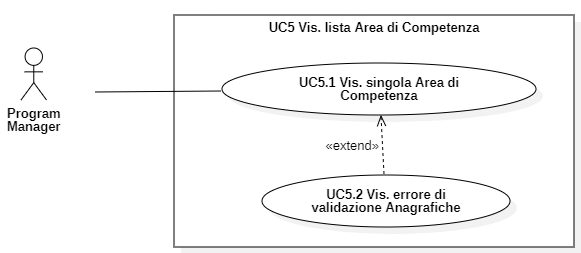
\includegraphics[width=0.6\columnwidth]{usecase/UC5} 
    \caption{Caso d'Uso 5 espanso}
\end{figure}
\begin{itemize}[label=$\circ$]
\item \textbf{Attore:} Program Manager;
\item \textbf{Descrizione:} il Program Manager può visualizzare la lista delle Aree di Competenza;
\item \textbf{Precondizioni:} il richiedente è un Program Manager;
\item \textbf{Postcondizioni:} la lista delle Aree di Competenza è visualizzabile dal Program Manager;
\item \textbf{Estensioni:} il caso d'uso non ha estensioni;
\item \textbf{Inclusioni:} il caso d'uso non ha inclusioni.
\end{itemize}

\subsubsection*{UC5.1 - Vis. singola Area di Competenza}
\begin{figure}[H] 
    \centering 
    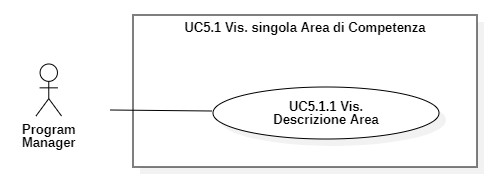
\includegraphics[width=0.6\columnwidth]{usecase/UC5.1} 
    \caption{Caso d'Uso 5.1 espanso}
\end{figure}
\begin{itemize}[label=$\circ$]
\item \textbf{Attore:} Program Manager;
\item \textbf{Descrizione:} il Program Manager può visualizzare un'Area di Competenza;
\item \textbf{Precondizioni:} il richiedente è un Program Manager;
\item \textbf{Postcondizioni:} l'Area di Competenza selezionata è visualizzabile dal Program Manager;
\item \textbf{Estensioni:}  UC5.2;
\item \textbf{Inclusioni:} il caso d'uso non ha inclusioni.
\end{itemize}

\subsubsection*{UC5.1.1 - Vis. descrizione Area}
\begin{itemize}[label=$\circ$]
\item \textbf{Attore:} Program Manager;
\item \textbf{Descrizione:} il Program Manager può visualizzare la descrizione di un'Area di Competenza;
\item \textbf{Precondizioni:}  l'Area è visualizzabile dal Program Manager;
\item \textbf{Postcondizioni:} il Program Manager può visualizzare la descrizione dell'Area di Competenza selezionata;
\item \textbf{Estensioni:} non ci sono estensioni;
\item \textbf{Inclusioni:} non ci sono inclusioni.
\end{itemize}

\subsubsection*{UC6 - Vis. lista Clienti}
\begin{figure}[H] 
    \centering 
    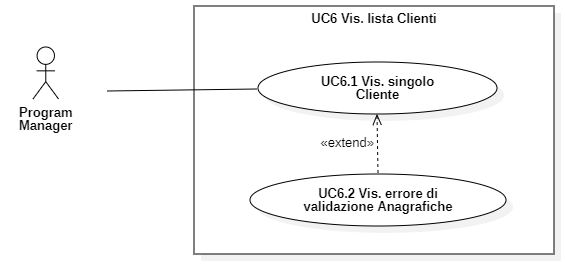
\includegraphics[width=0.6\columnwidth]{usecase/UC6} 
    \caption{Caso d'Uso 6 espanso}
\end{figure}
\begin{itemize}[label=$\circ$]
\item \textbf{Attore:} Program Manager;
\item \textbf{Descrizione:} il Program Manager può visualizzare la lista dei Clienti;
\item \textbf{Precondizioni:} il richiedente è un Program Manager;
\item \textbf{Postcondizioni:} la lista dei Clienti è visualizzabile dal Program Manager;
\item \textbf{Estensioni:} il caso d'uso non ha estensioni;
\item \textbf{Inclusioni:} il caso d'uso non ha inclusioni.
\end{itemize}

\subsubsection*{UC6.1 - Vis. singolo Cliente}
\begin{figure}[H] 
    \centering 
    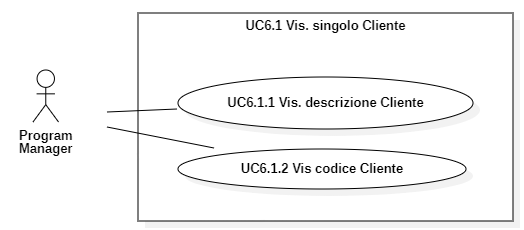
\includegraphics[width=0.6\columnwidth]{usecase/UC6.1} 
    \caption{Caso d'Uso 6.1 espanso}
\end{figure}
\begin{itemize}[label=$\circ$]
\item \textbf{Attore:} Program Manager;
\item \textbf{Descrizione:} il Program Manager può visualizzare un Cliente;
\item \textbf{Precondizioni:} il richiedente è un Program Manager;
\item \textbf{Postcondizioni:} il Cliente selezionato è visualizzabile dal Program Manager;
\item \textbf{Estensioni:} UC6.2;
\item \textbf{Inclusioni:} non ci sono inclusioni.
\end{itemize}

\subsubsection*{UC6.1.1 - Vis. descrizione Cliente}
\begin{itemize}[label=$\circ$]
\item \textbf{Attore:} Program Manager;
\item \textbf{Descrizione:} il Program Manager può visualizzare la descrizione di Cliente;
\item \textbf{Precondizioni:}  il Cliente è visualizzabile dal Program Manager;
\item \textbf{Postcondizioni:} il Program Manager può visualizzare la descrizione del Cliente selezionato;
\item \textbf{Estensioni:} il caso d'uso non ha estensioni;
\item \textbf{Inclusioni:} il caso d'uso non ha inclusioni.
\end{itemize}

\subsubsection*{UC6.1.2 - Vis. codice Cliente}
\begin{itemize}[label=$\circ$]
\item \textbf{Attore:} Program Manager;
\item \textbf{Descrizione:} il Program Manager può visualizzare il codice del Cliente;
\item \textbf{Precondizioni:} il Cliente è visualizzabile dal Program Manager;
\item \textbf{Postcondizioni:} il Program Manager può visualizzare il codice del Cliente selezionato;
\item \textbf{Estensioni:} il caso d'uso non ha estensioni;
\item \textbf{Inclusioni:} il caso d'uso non ha inclusioni.
\end{itemize}
